\title{Analysis of Java Based Open Source Projects}
\author{
         Cristina Videira Lopes\\
         \fontsize{10pt}{9.6pt}\selectfont
        \href{mailto:lopes@uci.edu}{\nolinkurl{lopes@uci.edu}}\\
         Abhinav Mukund Kulkarni\\
        \fontsize{10pt}{9.6pt}\selectfont
        \href{mailto:abhinav.kulkarni@uci.edu}{\nolinkurl{abhinav.kulkarni@uci.edu}}\\
        \fontsize{10pt}{9.6pt}\selectfont
        Bren School of Informatics \& Computer Sciences\\
        \fontsize{10pt}{9.6pt}\selectfont
        University of California, Irvine\\
}
\date{December 2012}

\documentclass[12pt]{article}

\usepackage[hidelinks]{hyperref}
\usepackage{inconsolata}
\usepackage{amsmath} 
\usepackage[pdftex]{graphicx}
\usepackage[center]{caption}
\usepackage{subcaption}
\usepackage{multirow}
\usepackage{array}
\usepackage{longtable}
\usepackage[toc,page]{appendix}
\usepackage{cite}

\begin{document}
\maketitle
\begin{abstract}
It is often of interest to study the evolution of a software project over time, compare two different projects by looking at their development histories and draw key summary statistics from the source code. It is also of use to know if there is any average trend in the development of projects and find out those projects that differ significantly from the average trend so that they can be studied closely to know what went different in their development proecesses. Matrices related to software development can also be used to make better estimation for upcoming projects.

In this report, we present an analysis of multiple Java based open-source projects of varying sizes and types. We draw heavily from a previous study related to Aspect Oriented Programming paradigm that suggests that software concerns and aspects can be modelled as latent topics in the source code.
\end{abstract}

\newpage
\section{Introduction}
Those involved in software developement and management often want to measure software development related matrices for the purpose of improving software quality and productivity. Also there is often a need to visualize the trajectory of the development of the project. In the next sections we detail techniques used to measure various matrices associated with software development process and draw several conclusions. Most of the techniques are drawn from a recent study related to Aspect Oriented Programming~\cite{Baldi:2008:TAL:1449955.1449807}.

Aspect Oriented Programming paradigm defines a concern as a cohesive area of functionality, such as logging, disk I/O or string handling. Usually a concern is spread across multiple classes and methods in source code files of a software project. Concerns are \emph{cross-cutting} in a sense that they cut across multiple abstractions. These concerns and aspects can be modelled as latent topics occuring in the source code and their cross-cutting and tangling can be precisely measured using entropies of probability distributions of topics over files and that of files over topics respectively~\cite{Baldi:2008:TAL:1449955.1449807}. Key summary statistics based on these entropies provide us with holistic view of the development process.

In the following sections we give a brief information about topic modelling and details about our experiemention with 24 Java based open-source projects and conclusions from the study.

\section{Topic Modelling}\label{Topic Modellig}
\subsection{Latent Dirichlet Distribution}\label{LDA}
Latent Dirichlet Allocation (LDA) is an unsupervised topic modelling techniques to find occurrences of abstract topics in a collection of documents~\cite{Blei:2003:LDA:944919.944937}. LDA treats documents as bag-of-words. It endows the entire collection with a Dirichlet distribution that picks out a multinomial probability vector of topics for each document. Within each document, for every word, a topic is selected according to the multinomial probability vector and then a word is generated according to a topic specific multinomial distribution over all the words. All of this can be expressed as following:\\
\\	
For each document $d$ in $D_{train}$:\\
Chose a topic probability vector $\vec\theta \sim$ Dir$(\vec\alpha)$\\
Chose a word probability vector $\vec\phi_t \sim$ Dir$(\vec\beta)$ for each topic $t$\\
For each word $w_{d_n}$ belonging to $d$:\\
\indent Select a topic $z_t \sim$ Multinomial$(\vec\theta)$\\
\indent Select a word $w_{dn} \sim$ Multinomial$(\vec\phi_t)$\\

Usually the Dirichlet priors on topic and word given topic probability distributions are symmetric. We used Gibbs sampling to learn the model parameters. Details about inference can be found in the original LDA publication~\cite{Blei:2003:LDA:944919.944937},~\cite{steyvers2007probabilistic}.

\subsection{LDA Software}\label{LDA Software}
We used couple of open-source packages to train topic models on the corpus of source code. Topic modelling toolbox by Mark Steyvers and Tom Griffiths is a MATLAB compliant software that can be used to train topic models~\cite{SteyversMATLAB}. It worked fine for all purposes, however we quickly ran into issues of scalability with bigger projects such as Eclipse, JBoss Drools and Netbeans and switched to Mallet, a Java-based open-source topic modelling toolkit~\cite{McCallumMALLET}. Mallet has a parallel topic modelling trainer.

\subsection{Finding Optimal Number of Topics}\label{Optimal Number of Topics}
We looked at projects of varyig sizes, complexity and development histories and it was important to find out natural number of topics for each version of each project before proceeding with any analysis. LDA literature has details about quite a few methodologies to determine natural number of topics occuring in a corpus, but most widely used one is based on calculating perplexity of test documents~\cite{Blei:2003:LDA:944919.944937}. We also considered another method that views LDA as a matrix factorization algorithm~\cite{arun2010finding} but decided to use perplexity measure as it provided clearer results and pinpoint estimate of natural number of topics.

\subsubsection{Perplexity} \label{Perplexity}
Document corpus is divided into training and test documents and perplexity is defined as:
\begin{equation*}
Perplexity(D_{test}|D_{train}) = exp\left\{-\frac{\sum_{d=1}^{M^{test}} \log p(\vec w_{d}|\mathbf{\Phi}, \alpha, \beta)}{\sum_{d=1}^{M^{test}} N_d}\right\}
\end{equation*}
\begin{equation*}
 = exp\left\{-\frac{\sum_{d=1}^{M_{test}} \log \int_{\vec\theta} p(\vec w_d|\vec\theta, \mathbf{\Phi}, \alpha)\cdot p(\vec{\theta}|\beta)\,\mathrm{d}\vec\theta}{\sum_{d=1}^{M^{test}} N_d}\right\}
\end{equation*}
\begin{equation*}
 = exp\left\{-\frac{\sum_{d=1}^{M_{test}} \log \int_{\vec\theta} \left\{p(\vec{\theta}|\beta)\prod_{n=1}^{N_d}p(w_{dn}|\vec\theta, \mathbf{\Phi}, \alpha)\right\}\,\mathrm{d}\vec\theta}{\sum_{d=1}^{M^{test}} N_d}\right\}
\end{equation*}
where $\vec w_d$ is $d^{th}$ document vector in the test corpus, $z_t$ is the $t^{th}$ topic, $M_{test}$ is the total number of documents in test corpus and last step follows from the fact that words in a document are independent give topic mixture for the document.\\

Above integration is hard to carry out over all possible multinomial topic assignments. With Stevyer's and Griffith's MATLAB topic modelling toolkit, we resorted to calculating ``half-document perplexity''~\cite{asuncion2012smoothing}. Instead of dividing corpus into training and test documents, we divide each document in training and test sections, learn topic mixture multinomial probability for each document during training phase and calculate perplexity on the test part of the document.
\begin{equation*}
Perplexity(D) = exp\left\{-\frac{\sum_{d=1}^M \log p(\vec w_{d}|\vec\theta_d, \mathbf{\Phi}, \alpha, \beta)}{\sum_{d=1}^M N_d}\right\}
\end{equation*}
\begin{equation*}
 = exp\left\{-\frac{\sum_{d=1}^M \sum_{n=1}^{N_d}\log p(w_{dn}|\vec\theta_d, \mathbf{\Phi}, \alpha, \beta)}{\sum_{d=1}^M N_d}\right\}
\end{equation*}
\begin{equation*}
 = exp\left\{-\frac{\sum_{d=1}^M \sum_{n=1}^{N_d}\log\left\{\sum_{t=1}^Tp(w_{dn}|\mathbf{\Phi}, \beta)\cdot p(z_t|\vec\theta_d, \alpha)\right\}}{\sum_{d=1}^M N_d}\right\}
\end{equation*}

Here topic probabilities for each document are known from training phase, hence there is no integration over $\vec\theta$. One alternative to above is to have separate training and test corpuses and run few iterations of Gibbs or Importance sampling on each test document to obtain corresponding topic mixtures~\cite{wallach2009evaluation}.\\
We used fixed values of $\alpha$ and $\beta$ for each project. While manually fixing their values introduces bias in the natural number of topics, it is a fairly common practice in topic modelling community to do so.

With Mallet, we used its in-build functionality for calculating perplexity on test corpus.

Wallach, et. al. 2009 has more details about evalutation methods for topic models~\cite{wallach2009evaluation}.

Figure~\ref{ppx1} and~\ref{ppx2} show perplexity graphs for selected versoins of Apache Ant and Lucene. It can be easily seen that perplexity graphs stabilize or rise upwards after reaching natural number of topics.
\begin{figure}
        \centering
        \begin{subfigure}[b]{0.5\textwidth}
                \centering
                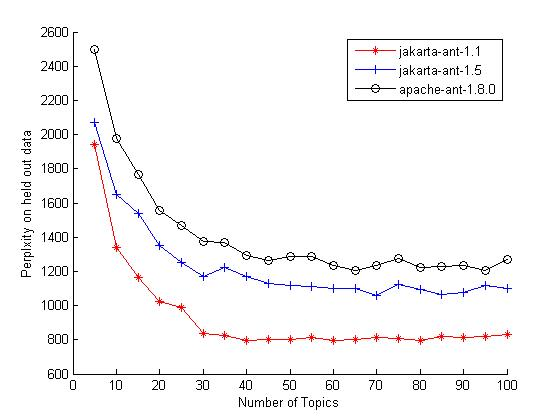
\includegraphics[width=\textwidth]{perplexity-ant.jpg}
                \caption{Perplexity plot for selected versions of Apache Ant}
                \label{ppx1}
        \end{subfigure}%
        \begin{subfigure}[b]{0.5\textwidth}
                \centering
                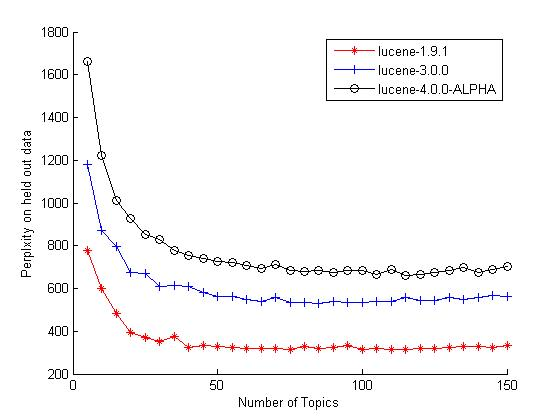
\includegraphics[width=\textwidth]{perplexity-lucene.jpg}
                \caption{Perplexity plot for selected versions of Apache Lucene}
                \label{ppx2}
        \end{subfigure}
        \begin{subfigure}[b]{\textwidth}
                \centering
                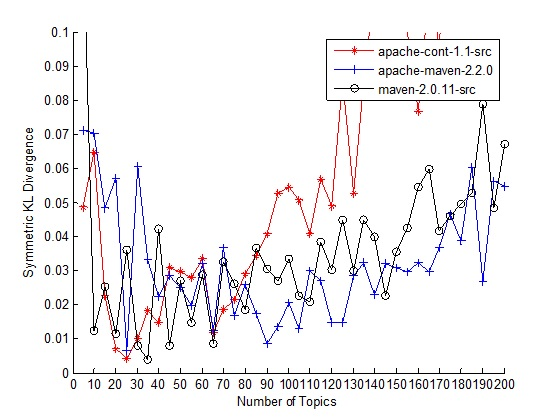
\includegraphics[width=\textwidth]{KL-divergence-maven.jpg}
                \caption{Symmetric KL divergence plot for selected versions of Apache Maven}
                \label{ppx3}
        \end{subfigure}
        \caption{Estimation of natural number of topics}\label{fig:numtopics}
\end{figure}

\subsubsection{Symmetric KL Divergence} \label{Symmetric KL Divergence}
The other method to find out natural number of topics is based on an idea that views LDA as a matrix factorization method and computes natural number of topics by maximizing ``quality of split'' (i.e. matrix factorization)~\cite{arun2010finding}. Unlike preplexity, this method highlights a range in which natural number of topics lies. Figure~\ref{ppx3} shows plot for Apache Maven. It is easy to see a dip for each version in the range 30-90.

\subsection{LDA Results} \label{LDA Results}
We analyzed 
Below are listed some of the topics extracted from different projects. It is not difficult to recognize that they represent specific functionalities such as string handling, I/O, etc. in Java.

\begin{center}
\begin{longtable}{|>{\small}m{7.1cm}|>{\small}m{3cm}|>{\small}c|}
\hline
\multicolumn{1}{|c|}{Top Words} & \multicolumn{1}{|c|}{Topic} & \multicolumn{1}{|c|}{Project} \\ \hline
\endhead
file buildexception io dest fileinputstream close length line & File I/O & Apache Ant \\ \hline
stringtokenizer tok nexttoken hasmoretokens token max path & String Tokenization & Apache Ant \\ \hline
swt bounds width x height y rectangles left & SWT GUI Functionalities & Eclipse \\ \hline
server port fetchpage mortbay startserver listener getserver socketlistener & Server Messaging & Apache Nutch \\ \hline
message cause protocolexception protocol suppresswarnings httpauthenticationexception ftpexception urlfilterexception parseexception & Protocol Exception Handling & Apache Nutch \\ \hline
dateformat timezone date format dateformattype dateformatoption timezoneid absolutetimedateformat equalsignorecase time settimezone & Date/Timezone Operations & Log4J \\ \hline
assertequals test assert conf asserttrue junit configuration class mockito org assertfalse fail set testcase & Assert/Testing & Apache Hadoop \\ \hline
taskid taskattemptid jobid job this taskstatus status task tasktracker jvmid counters id tip jobinprogress get jobstatus state tracker taskinprogress & Hadoop Job/Task Tracking & Apache Hadoop \\ \hline
mapper reducer name outputpath log inputpath argmap outputformat inputformat writable catfile mainclasses mappervalue mapperkey & Hadoop Map/Reduce & Apache Mahout \\ \hline
\end{longtable}
\end{center}

\section{Source Code Analysis}\label{Source Code Analysis}
We draw a number of key summary statistics from the corpus. In particular, we focussed on minor releases for each project (such as v1.1, v1.2, v2.1, v2.2, etc.). Source code for each version was tokenized and obvious Java and project-specific stopwords were removed. A topic model for each version was fit with natural number of topics obtained from previous analysis. The details about each project are presented in Appendix A. It can be seen that the natural number of topics roughly correlates with project size.

\subsection{Topic Scattering}
Topic scattering is the entropy of the distribution of a topic over documents. We calculated mean topic scattering for each version (summation of topic entropies weighted by probability of occurrence of the topics). Topic entropy can be viewed as a measure of localization of the cohesive functionlity that the topic represents. Higher the entropy, higher the spread of aspect over large parts of source code. Please refer to Baldi, Lopes, et. al. (2008)~\cite{Baldi:2008:TAL:1449955.1449807} for more discussion about topic scattering.
For almost all projects, mean normalized scattering increases over time as projects evolve and become complex (figure~\ref{scatter1} and~\ref{scatter2}). There are a few exceptions such as CoffeeMud project as depicted in figure~\ref{scatter3} and~\ref{scatter4}.
\begin{figure}
        \centering
        \begin{subfigure}[b]{0.5\textwidth}
                \centering
                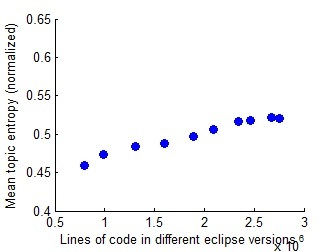
\includegraphics[width=\textwidth]{mean-scattering-vs-loc-eclipse.jpg}
                \caption{Mean topic scattering against LOC of Eclipse versions}
                \label{scatter1}
        \end{subfigure}%
        \begin{subfigure}[b]{0.5\textwidth}
                \centering
                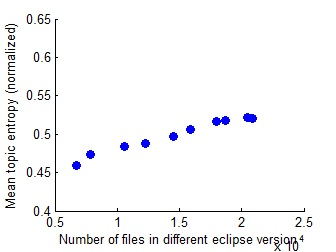
\includegraphics[width=\textwidth]{mean-scattering-vs-num-files-eclipse.jpg}
                \caption{Mean topic scattering against number of files in Eclipse versions}
                \label{scatter2}
        \end{subfigure}
        \begin{subfigure}[b]{0.5\textwidth}
                \centering
                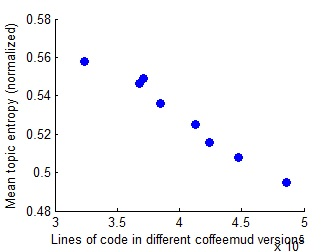
\includegraphics[width=\textwidth]{mean-scattering-vs-loc-coffeemud.jpg}
                \caption{Mean topic scattering against LOC of CoffeeMud versions}
                \label{scatter3}
        \end{subfigure}%
        \begin{subfigure}[b]{0.5\textwidth}
                \centering
                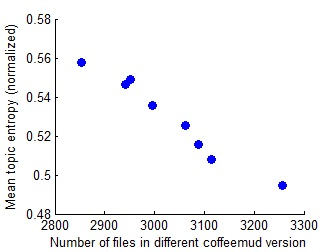
\includegraphics[width=\textwidth]{mean-scattering-vs-num-files-coffeemud.jpg}
                \caption{Mean topic scattering against number of files in CoffeeMud versions}
                \label{scatter4}
        \end{subfigure}
        \caption{Mean topic scattering over time}\label{fig:scattering}
\end{figure}

\subsection{File Tangling}
File tangling is the entropy of the distribution of a file over topics. We calculated average file tangling for each version. File tangling can be viewed as a measure of heterogeneity of a souce code document in terms of concerns. Please refer to Baldi, Lopes, et. al. (2008)~\cite{Baldi:2008:TAL:1449955.1449807} for more discussion about file tangling.
For almost all projects, average normalized file tangling increases over time as projects evolve and become complex (figure~\ref{tangle1} and~\ref{tangle2}). There are a few exceptions such as CoffeeMud as in figure~\ref{tangle3} and~\ref{tangle4}.
\begin{figure}
        \centering
        \begin{subfigure}[b]{0.5\textwidth}
                \centering
                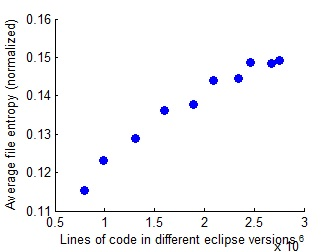
\includegraphics[width=\textwidth]{average-tangling-vs-loc-eclipse.jpg}
                \caption{Average file tangling against LOC of Eclipse versions}
                \label{tangle1}
        \end{subfigure}%
        \begin{subfigure}[b]{0.5\textwidth}
                \centering
                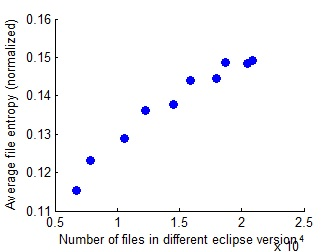
\includegraphics[width=\textwidth]{average-tangling-vs-num-files-eclipse.jpg}
                \caption{Average file tangling against number of files in Eclipse versions}
                \label{tangle2}
        \end{subfigure}
        \begin{subfigure}[b]{0.5\textwidth}
                \centering
                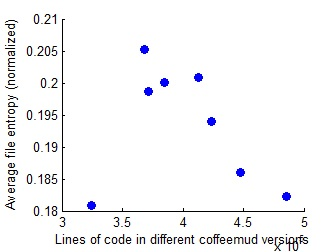
\includegraphics[width=\textwidth]{average-tangling-vs-loc-coffeemud.jpg}
                \caption{Average file tangling against LOC of CoffeeMud versions}
                \label{tangle3}
        \end{subfigure}%
        \begin{subfigure}[b]{0.5\textwidth}
                \centering
                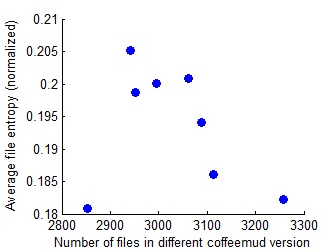
\includegraphics[width=\textwidth]{average-tangling-vs-num-files-coffeemud.jpg}
                \caption{Average file tangling against number of files in CoffeeMud versions}
                \label{tangle4}
        \end{subfigure}
        \caption{Average file tangling over time}\label{fig:tangling}
\end{figure}

\subsection{Overall Statistics} \label{Overall Statistics}
Figure~\ref{fig:overall} shows mean scattering and average tangling of all project versions. It is easy to spot upward trend.
\begin{figure}
        \centering
        \begin{subfigure}[b]{0.5\textwidth}
                \centering
                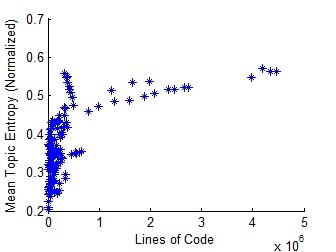
\includegraphics[width=\textwidth]{mean-scattering-vs-loc-overall.jpg}
                \caption{Average mean scattering against LOC of different versions}
                \label{overall-scatter1}
        \end{subfigure}%
        \begin{subfigure}[b]{0.5\textwidth}
                \centering
                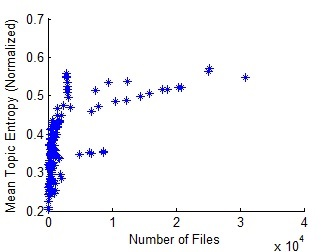
\includegraphics[width=\textwidth]{mean-scattering-vs-num-files-overall.jpg}
                \caption{Average mean scattering against number of files in different versions}
                \label{overall-scatter2}
        \end{subfigure}
        \begin{subfigure}[b]{0.5\textwidth}
                \centering
                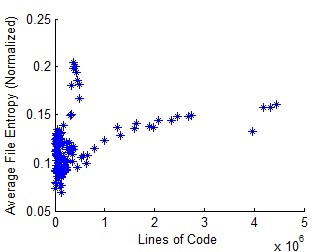
\includegraphics[width=\textwidth]{average-tangling-vs-loc-overall.jpg}
                \caption{Average file tangling against LOC of different versions}
                \label{overall-tangle1}
        \end{subfigure}%
        \begin{subfigure}[b]{0.5\textwidth}
                \centering
                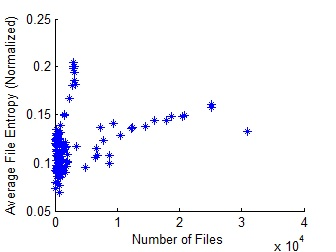
\includegraphics[width=\textwidth]{average-tangling-vs-num-files-overall.jpg}
                \caption{Average file tangling against number of files in different versions}
                \label{overall-tangle2}
        \end{subfigure}
        \caption{Overall Statistics}\label{fig:overall}
\end{figure}

%%%%%%%%%%%%%%%%%%%%%%%%%%%%%%%%%%%%%%%%%%%%%%%%%%%%%%%%%%%%%%%%%%%%%%

\begin{figure}
        \centering
        \begin{subfigure}[b]{0.5\textwidth}
                \centering
                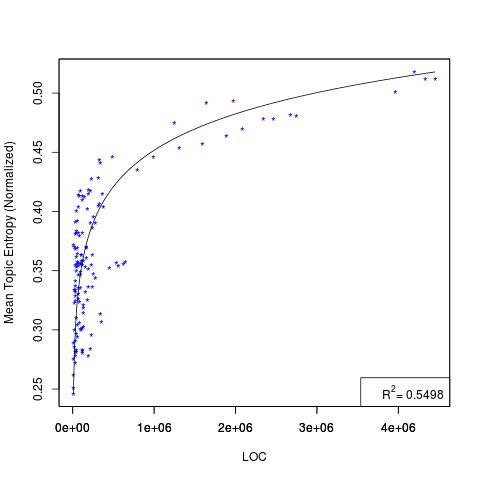
\includegraphics[width=\textwidth]{mean-scattering-vs-loc-overall-fitted.jpg}
                \caption{Mean scattering against LOC of different versions}
                \label{overall-scatter1}
        \end{subfigure}%
        \begin{subfigure}[b]{0.5\textwidth}
                \centering
                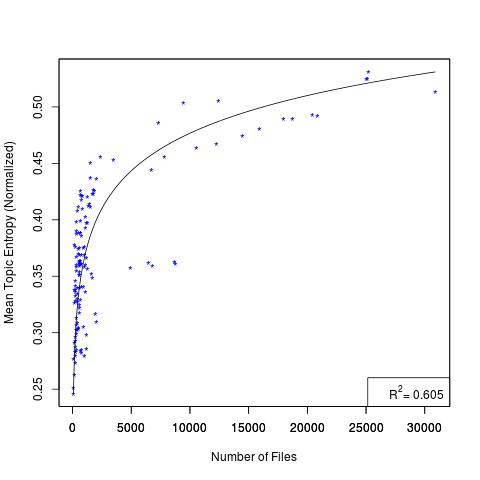
\includegraphics[width=\textwidth]{mean-scattering-vs-num-files-overall-fitted.jpg}
                \caption{Mean scattering against number of files in different versions}
                \label{overall-scatter2}
        \end{subfigure}
        \begin{subfigure}[b]{0.5\textwidth}
                \centering
                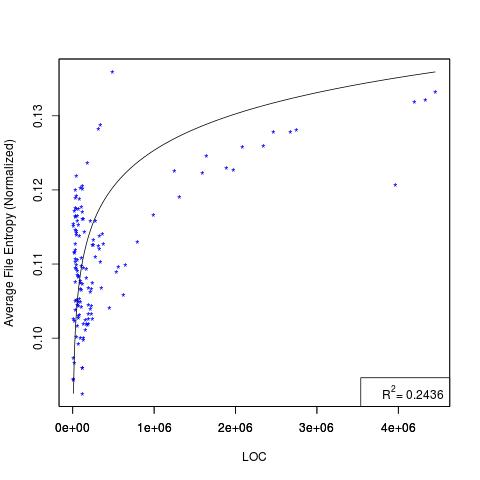
\includegraphics[width=\textwidth]{average-tangling-vs-loc-overall-fitted.jpg}
                \caption{Average file tangling against LOC of different versions}
                \label{overall-tangle1}
        \end{subfigure}%
        \begin{subfigure}[b]{0.5\textwidth}
                \centering
                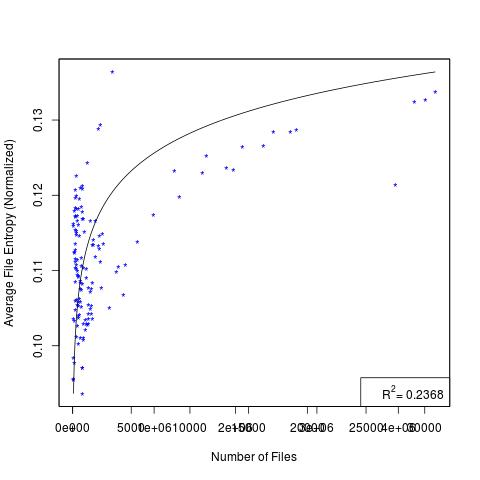
\includegraphics[width=\textwidth]{average-tangling-vs-num-files-overall-fitted.jpg}
                \caption{Average file tangling against number of files in different versions}
                \label{overall-tangle2}
        \end{subfigure}
        \caption{Fitted Curves for Overall Statistics}\label{fig:overall2}
\end{figure}

%%%%%%%%%%%%%%%%%%%%%%%%%%%%%%%%%%%%%%%%%%%%%%%%%%%%%%%%%%%%%%%%%%%%%%

\section{Conclusion}
Figure~\ref{fig:overall2} shows fitted curves obtained by fitting mean scattering/average tangling with log of LOC/number of files. We obtained following fit:
\[ MeanScattering = -0.16 + 0.044\cdot\log{(LOC)}\;\;\;\;\;\;\;\;{(R^2 = 0.5498)}\]
\[ MeanScattering = 0.03 + 0.048\cdot\log{(NumFiles)}\;\;\;\;\;\;\;\;(R^2 = 0.605)\]
The plots for average tangling do not quite lend themselves to a good linear model fit against logarithm of LOC/number of files, however the trend is not very different from that observed in case of mean scattering.

Standard statistical tests can be employed to identify outlying projects/versions for further analysis.

\newpage
\bibliography{bibtex}{}
\bibliographystyle{plain}

\newpage
%\appendixpage
%\renewcommand{\appendixname}{Project Details}
%\section{Project Details}
\end{document}